\clearpage
\section{So sánh, trực quan hóa và khai phá tri thức}
\subsection{Trực quan hóa và So sánh hiệu năng}
% Bảng/Biểu đồ so sánh độ chính xác (R-squared, RMSE) giữa mô hình Linear Regression (Đề cương) và Random Forest (Nâng cao) để chứng minh sự cải thiện.

Để đánh giá hiệu quả của việc áp dụng các kỹ thuật học máy nâng cao, nhóm tiến hành so sánh hiệu năng giữa mô hình cơ sở (Baseline Model - Linear Regression) và mô hình nâng cao (Advanced Model - Random Forest).\medskip

Mô hình hồi quy tuyến tính đơn giản (chỉ sử dụng \texttt{GrLivArea}) cho thấy mức độ giải thích dữ liệu ở mức trung bình với $R^2 \approx 0.5402$ và sai số RMSE lên đến 58,137.54 USD. Điều này phản ánh rõ hạn chế của việc chỉ sử dụng một đặc trưng diện tích đơn lẻ để dự đoán một biến mục tiêu phức tạp như giá nhà.\medskip

Ngược lại, mô hình Random Forest (với tập đặc trưng đa dạng và khả năng nắm bắt các mối quan hệ phi tuyến tính) đã cải thiện đáng kể các chỉ số đánh giá. Việc giảm mạnh RMSE và tăng $R^2$ chứng minh rằng thuật toán tập hợp (Ensemble Learning) giúp mô hình học được các mẫu phức tạp hơn, tránh hiện tượng quá khớp (overfitting) nhờ cơ chế lấy mẫu ngẫu nhiên (bootstrap) và kết hợp nhiều cây quyết định.

\begin{figure}[h]
    \centering
    
\includegraphics[width=0.9\textwidth]{images/results/model_comparison.png}
    \caption{Biểu đồ so sánh hiệu năng (RMSE và R-squared) giữa Linear Regression và Random Forest}
    \label{fig:model_comparison}
\end{figure}

\subsection{Khai phá tri thức}
%Phân tích và trực quan hóa các đặc trưng có sức ảnh hưởng lớn nhất đến SalePrice (OverallQual, TotalSF, GrLivArea...).
Thông qua thuộc tính \texttt{feature\_importances\_} của mô hình Random Forest, nhóm đã trích xuất và đo lường mức độ đóng góp của từng đặc trưng đối với giá trị căn nhà (\texttt{SalePrice}).

\begin{figure}[h]
\centering
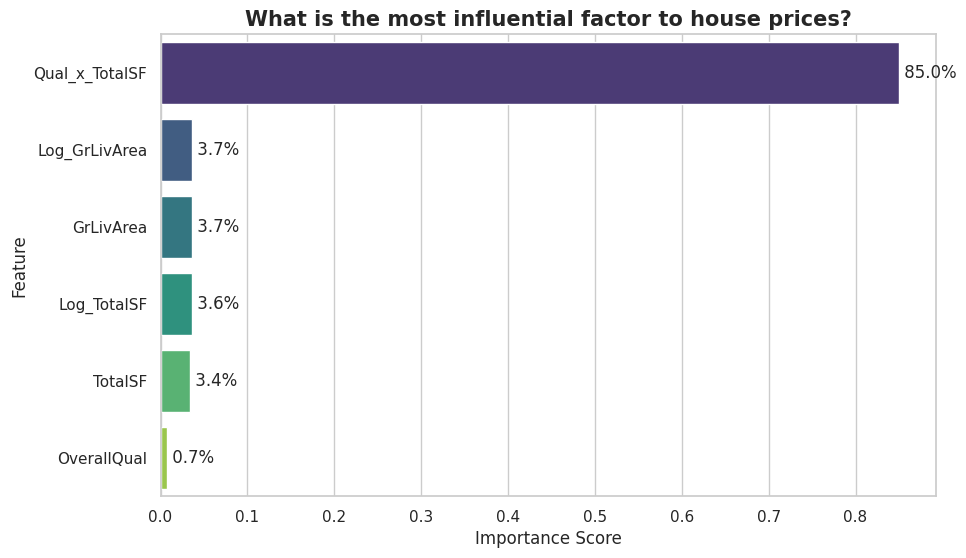
\includegraphics[width=0.8\textwidth]{images/results/feature_importance.png}
\caption{Trực quan hóa mức độ quan trọng của các đặc trưng (Feature Importance)}
\label{fig:feature_importance}
\end{figure}

Kết quả phân tích cho thấy sự phân hóa rõ rệt:
\begin{itemize}
\item \textbf{Biến kết hợp (\texttt{Qual\_x\_TotalSF}) giữa chất lượng tổng thể (\texttt{OverallQual}) và tổng diện tích sử dụng ngôi nhà (\texttt{TotalSF}):} Đây là đặc trưng mang tính quyết định lớn nhất, chiếm hơn 85\% mức độ ảnh hưởng đến giá nhà. Điều này cho thấy yếu tố thẩm mỹ, vật liệu hoàn thiện và tình trạng bảo trì đóng vai trò then chốt trong định giá bất động sản.
\item \textbf{Các yếu tố về diện tích (\texttt{TotalSF}, \texttt{GrLivArea}):} Diện tích sử dụng thực tế (đặc biệt là không gian sống trên mặt đất và tổng diện tích khu vực) là nhóm yếu tố có ảnh hưởng đáng kể. Không gian rộng rãi thường đi kèm với giá trị cơ bản của bất động sản.
\item \textbf{Tối ưu nguồn lực dữ liệu:} Hệ thống định giá thực tế có thể dự đoán chính xác giá nhà chỉ bằng cách tập trung vào top 6-10 thông số quan trọng nhất thay vì phải thu thập toàn bộ hơn 80 biến số ban đầu. Việc này giúp tiết kiệm đáng kể chi phí thu thập và xử lý dữ liệu.
\end{itemize}
